\section{Introduction}
\label{sec:intro}

Projection methods protect an old task by writing the new one only in directions the old task does not use~\citep{zeng2019owm,farajtabar2020ogd,saha2021gpm}.
They treat the old weights as something to avoid.
Information theory suggests a different stance.
When a channel adds interference that the transmitter knows in advance, Costa showed that the capacity equals that of a channel with no interference at all~\citep{costa1983,gelfand1980}: the transmitter precodes around the interference instead of cancelling it.
A continual learner knows its old weights exactly, so the analogy proposes \emph{dirty-paper writes}: precode the new task's update against the old weights, and old knowledge should cost no write capacity.

The theorem needs more than known interference; it needs a decoder that folds the signal modulo a lattice~\citep{erez2005lattice}.
Ordinary readouts are not periodic, and for them the precoding coset collapses to a single point and the dirty-paper write is GPM (\cref{sec:scope}).
We therefore build the most favorable case: a two-layer ReLU network whose readout labels are residues modulo \(M=8\), so that every lattice precoder from communications applies verbatim.
If dirty-paper writes cannot beat projection here, they cannot beat it with a standard decoder.

The premise holds (\cref{tab:main}): the best precoded write's norm is within 7\% of an interference-free write's at every interference level, while GPM pays up to \gpmcleanmax{} times more when the old outputs span several periods.
The proposed gain does not follow.
\Cref{fig:budget} shows why at the main configuration: the same coset freedom is available to GPM by descending the periodic loss, and that baseline reaches the same new-task accuracy at every norm.
The joint precoder that moves old outputs by whole periods is the only arm that writes with markedly less norm, and it pays for the saving with old-task accuracy below its threshold.
Our contributions are:
\begin{itemize}
  \item a matched test of dirty-paper writes against GPM, OWM and GPM with modular descent at 15 equal update norms, \nconfigs{} configurations and \nseeds{} seeds, with a pre-registered kill bar (\cref{sec:method});
  \item a negative result: the dirty-paper arms do not beat projection on old-task accuracy anywhere and fail the new-task bar in \nkilled{} of \nconfigs{} configurations (\cref{sec:results});
  \item the exact place where the analogy breaks: Costa's saving survives, but it is a saving in write norm, which a cheaper modular descent mostly recovers and which the one arm that keeps it converts into a retention cliff (\cref{sec:scope}).
\end{itemize}

\begin{figure}[!t]
  \centering
  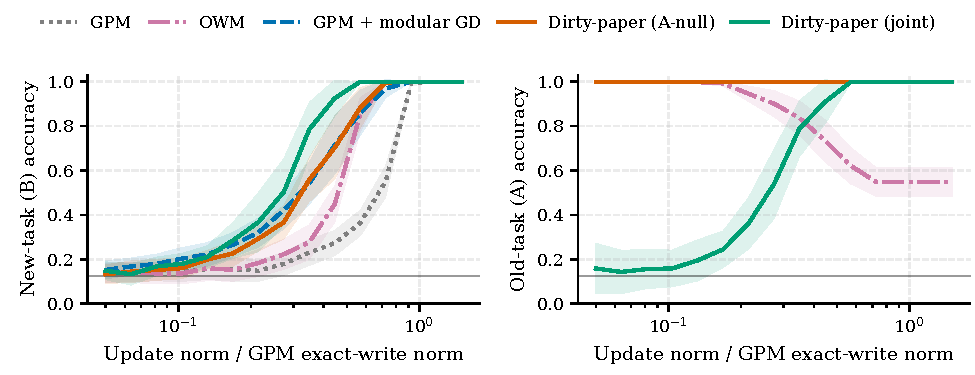
\includegraphics[width=\textwidth]{budget.pdf}
  \caption{\textbf{At equal update norm, dirty-paper writes do not beat projection.}
  Main configuration (\(\vartheta=30^\circ\), \(S=0\)); the horizontal axis is the update norm as a fraction of GPM's exact-write norm.
  Left: new-task accuracy. The A-null dirty-paper write tracks GPM with modular descent at every norm. The joint write learns earlier.
  Right: old-task accuracy. Every A-null arm keeps 100\%, so no write can beat GPM on the primary metric. The joint write and OWM lose old items when the norm is short.
  Lines are means over \nseeds{} seeds, bands 95\% Student-\(t\) intervals, and the gray line is chance (\(1/8\)).}
  \label{fig:budget}
\end{figure}
